Este guia sintetiza os conhecimentos que são necessários para trabalhar com a nova arquitetura 
Erlangms no ambiente Java. Este trabalho é resultado dos esforços realizados no Mestrado em Computação 
Aplicada pelo Analista Everton de Vargas Agilar do CPD/UnB.

Parta adiantar, a abordagem proposta por esta arquitetura
impõem o uso de um barramento de serviço desenvolvido na 
linguagem Erlang e um SDK (Software Development Kit) na linguagem 
que será utilizada para a implementação dos Web-Services, neste caso, o SDK ems-java 
para a linguagem Java. 

De forma muito resumida, a arquitetura ErlangMS tem o intuíto de facilitar a 
criação e a integração de sistemas através de uma abordagem
orientada a serviços no estilo arquitetural REST (Representational State Transfer). 
Não se preocupe, este estilo não é mais do que um conjunto de restrições que devemos 
seguir do que uma nova tecnologia. Assim, usa-se 
os verbos HTTP para realizar as operações desejadas, como por exemplo, o verbo POST para incluir
ou cadastrar alguma coisa, o verbo PUT para alterar, o verbo GET para pesquisar e o 
DELETE para excluir.

Em uma arquitetura como esta, existe a figura do Front-end (a parte visual do sistema) 
e o Back-end (a parte onde estão as regras de negócios providos através de serviços).



\section{Componentes em Tempo de Execução}

Os principais componentes da arquitetura em tempo de execução estão listados a seguir
com uma breve descrição sobre o seu objetivo sem entrar em muitos detalhes:


\subsection{Barramento de serviços (ems-bus)}

Sua função é interligar os clientes (tipicamente os Front-ends) 
aos serviços que contém as regras de negócios da organização. Quando alguém faz uma requisição
para um serviço, é o barramento que intermedia o envio e o recebimento das mensagens, sendo que o cliente
só precisa saber o endereço do barramento para isso.

\begin{figure}[htb]
\centering
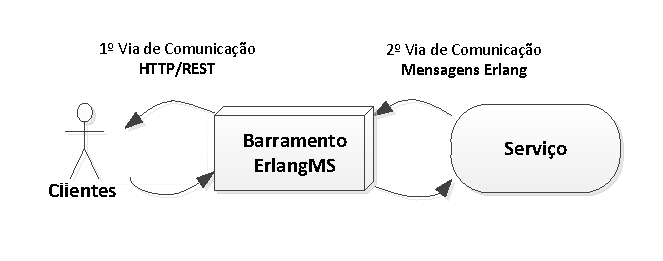
\includegraphics[scale=1.2]{/img/arquitetura/roteamento_mensagens.pdf}
\caption{Esquema do roteamento das mensagens da arquitetura.}
\label{fig:roteamento_mensagens}
\end{figure}
\FloatBarrier


\subsection{Catálogo de serviços}

Representa o componente chave da arquitetura pois permite
dar visibilidade aos serviços disponibilizados na organização. É no catálogo que 
os serviços são registrados. O exemplo a seguir expõem um serviço no catálogo 
para incluir uma resposta para um estudo preliminar do sistema SAE da UnB.


\lstset{
        basicstyle=\footnotesize,
        numbers=left,
        numberstyle=\footnotesize,
        tabsize=2,
        numbers=none,
        rulesepcolor=\color{blue}}
\renewcommand{\lstlistingname}{Código}             
\begin{lstlisting}[caption=Exemplo de um serviço no catálogo de serviços., label=fig:catalogo_processo] 
{
  "name": "/sae/estudo/preliminar/:id/resposta",
	"comment": "Cadastrar resposta do estudo preliminar",
	"owner": "sae",
	"service" : "br.unb.sae.facade.EstudoPreliminarFacade:insertResposta",
	"url": "/sae/estudo/preliminar/:id/resposta",
	"type": "POST"
}
\end{lstlisting}


\subsection{Módulo Back-end}

È um projeto Java Web típico do CPD/UnB
mas desenvolvido com um padrão de design que será apresentado mais adiante neste 
guia e que contém a implementação dos serviços. No CPD, estes projetos
são publicados em servidores de aplicação JBoss/Wildfly.

\subsection{Módulo Front-end}

Consiste na interface da aplicação bem como a parte que o usuário vê. O front-end é o responsável por coletar os dados de entrada do usuário
e realizar as chamadas para os serviços por meio do barramento de serviços.

\subsection{Servidor de Aplicação JBoss/Wildfly}

O servidor de aplicação JBoss/Wildfly é onde são publicados (deployment)
os projetos Java Web. Podem existir várias instâncias desses servidores para
aumentar a escalabilidade dos serviços, sendo que o barramento despacha
as requisições dos clientes utilizando um simples algoritmo round-robin.

\subsection{Erlang Port Mapper Daemon}

É um serviço que executa em 
segundo plano em cada nó de um cluster e que age como um servidor de nome.
É importante salientar que tanto o barramento quanto os
servidores de aplicação JBoss/Wildfly são vistos como nós 
na arquitetura. O cliente não faz parte do cluster pois é apenas um consumidor.

